\chapter{Лагранжианы, поля и локальные процессы с частицами}

Бозонные поля, фермионные поля и электромагнитное поле подчиняются уравнениям волнового типа. Эти уравнения содержат сами поля вместе с их производными по пространству и времени. Можно было бы выписать отдельное уравнение движения для каждого поля, но лагранжиан собирает всю систему в одно компактное выражение. Применение правила Эйлера--Лагранжа к этому выражению сразу дает уравнения для всех полей.

Эта конструкция тесно связана с принципом стационарного действия. Непосредственная задача здесь более конкретна: выяснить, от чего зависит лагранжиан поля, использовать его, чтобы получить несколько классических уравнений, а затем переосмыслить те же полевые выражения квантовомеханически. В квантовой теории лагранжиан управляет движением и взаимодействием частиц и, в конечном счете, амплитудами и сечениями столкновений.

\section{Компактная запись уравнений поля}

Для одного скалярного поля плотность лагранжиана зависит от самого поля и от его первых производных,
\begin{equation}
\mathcal L
=
\mathcal L\!\left(\phi,\partial_t\phi,\partial_x\phi,\ldots\right)
=
\mathcal L\!\left(\phi,\partial_\mu\phi\right).
\end{equation}
При вычислениях явное перечисление временной и пространственных производных часто полезнее; обозначение \(\partial_\mu\phi\) упаковывает тот же список в релятивистскую форму.

\begin{figure}[htbp]
\centering
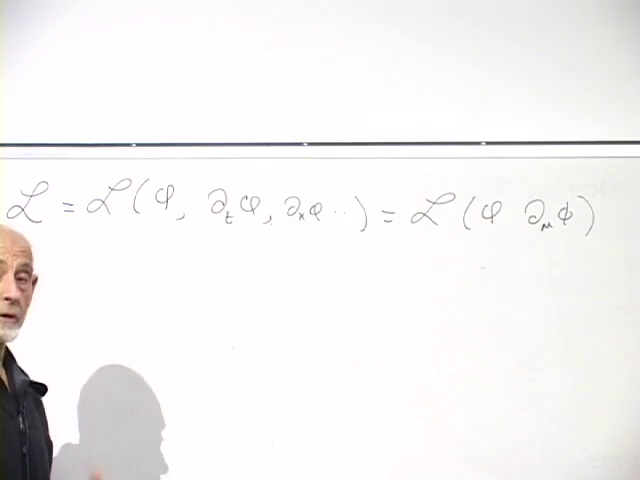
\includegraphics[width=0.82\textwidth]{lecture_09_figure_03.png}
\caption{Зависимость лагранжиана скалярного поля от поля и его пространственно-временных производных.}
\lectureframe{00:03:56}
\end{figure}

Уравнение Эйлера--Лагранжа для поля имеет вид
\begin{equation}
\frac{\partial}{\partial t}
\frac{\partial\mathcal L}{\partial\dot\phi}
+
\frac{\partial}{\partial x}
\frac{\partial\mathcal L}{\partial\phi_x}
+
\frac{\partial}{\partial y}
\frac{\partial\mathcal L}{\partial\phi_y}
+
\frac{\partial}{\partial z}
\frac{\partial\mathcal L}{\partial\phi_z}
=
\frac{\partial\mathcal L}{\partial\phi},
\end{equation}
где
\begin{equation}
\dot\phi=\frac{\partial\phi}{\partial t},
\qquad
\phi_x=\frac{\partial\phi}{\partial x},
\qquad
\phi_y=\frac{\partial\phi}{\partial y},
\qquad
\phi_z=\frac{\partial\phi}{\partial z}.
\end{equation}
Если \(\mathcal L\) содержит несколько полей, это правило применяется по одному разу к каждому полю. В результате получается система уравнений движения.

Простейший скалярный пример имеет вид
\begin{equation}
\begin{split}
\mathcal L
&=
\frac12\dot\phi^2
-\frac12\phi_x^2
-\frac12\phi_y^2
-\frac12\phi_z^2
-V(\phi)
\\
&=
\frac12\dot\phi^2-\frac12(\boldsymbol\nabla\phi)^2-V(\phi).
\end{split}
\end{equation}
Члены с пространственными производными имеют знак, противоположный знаку члена с временной производной. Дифференцируя по членам, получаем
\begin{align}
\frac{\partial\mathcal L}{\partial\dot\phi}&=\dot\phi,
&
\frac{\partial\mathcal L}{\partial\phi_i}&=-\phi_i,
&
\frac{\partial\mathcal L}{\partial\phi}&=-V'(\phi),
\end{align}
и, следовательно,
\begin{equation}
\ddot\phi-\nabla^2\phi=-V'(\phi).
\end{equation}

\begin{figure}[htbp]
\centering
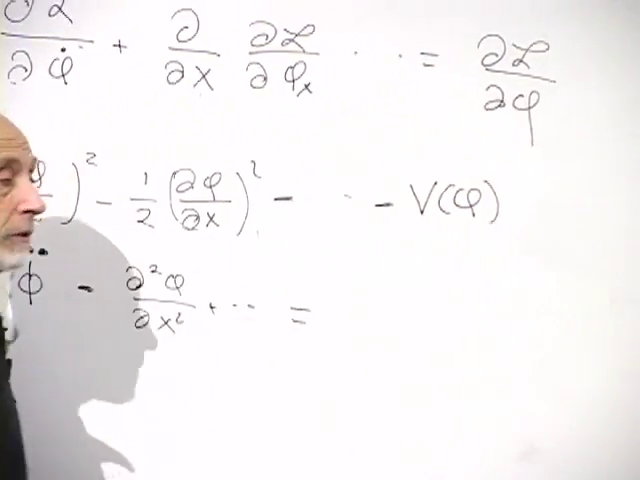
\includegraphics[width=0.74\textwidth]{lecture_09_figure_04.png}
\caption{Уравнение Эйлера--Лагранжа, лагранжиан скалярного поля и уравнение поля, порождаемое \(V(\phi)\).}
\lectureframe{00:08:23}
\end{figure}

Это уравнение, порождаемое скалярным лагранжианом.\editorialnote{Сохраненный кадр обрезан по левому краю; показанное завершение определяется непосредственно окружающим устным выводом.}

Здесь \(V(\phi)\) — плотность потенциальной энергии поля. Постоянный вклад в \(V\) не влияет на это уравнение, потому что его производная обращается в нуль. Линейный потенциал алгебраически возможен, но у него нет нижней границы: энергия поля может уходить к отрицательной бесконечности. Поэтому первым устойчивым примером является
\begin{equation}
V(\phi)=\frac12m^2\phi^2,
\qquad
V'(\phi)=m^2\phi,
\end{equation}
что дает
\begin{equation}
\ddot\phi-\nabla^2\phi=-m^2\phi.
\end{equation}

Чтобы выявить смысл \(m\), подставим плоскую волну,
\begin{equation}
\phi(\mathbf x,t)=\phi_0e^{i\omega t-i\mathbf k\cdot\mathbf x}.
\end{equation}
Тогда
\begin{equation}
\ddot\phi=-\omega^2\phi,
\qquad
\nabla^2\phi=-\mathbf k^2\phi,
\end{equation}
так что волновое уравнение принимает вид
\begin{equation}
-\omega^2\phi+\mathbf k^2\phi=-m^2\phi.
\end{equation}
После сокращения на \(\phi\),
\begin{equation}
\omega^2=\mathbf k^2+m^2.
\end{equation}
В единицах, где \(\hbar=c=1\), частота есть энергия, а волновое число — импульс. Следовательно,
\begin{equation}
E^2=\mathbf p^2+m^2,
\end{equation}
или, при восстановлении степеней \(c\), \(E^2=\mathbf p^2c^2+m^2c^4\). Параметр \(m\) есть масса одного кванта поля.

Релятивистскую инвариантность можно наложить на уровне компактного выражения. Если \(\mathcal L\) является лоренцевским скаляром, то его уравнения движения лоренц-инвариантны. Относительный знак между временными и пространственными производными — это привычное пространственно-временное соотношение знаков специальной теории относительности.

\section{Нелинейность и связанные классические поля}

Более высокие степени поля вводят новый тип поведения. Если
\begin{equation}
V(\phi)=\frac12m^2\phi^2+g\phi^3,
\end{equation}
то
\begin{equation}
\ddot\phi-\nabla^2\phi=-m^2\phi-3g\phi^2.
\end{equation}
Квадратичные члены в лагранжиане дают уравнения, линейные по полю. Кубические и более высокие члены дают нелинейные уравнения.

Различие видно в движении волновых пакетов. Для линейного уравнения пакет, движущийся вправо, и пакет, движущийся влево, можно сложить, получив еще одно решение. Они некоторое время перекрываются и интерферируют, затем проходят друг сквозь друга и выходят с исходными формами. При наличии нелинейных членов пакеты влияют друг на друга. Они могут рассеиваться, деформироваться или распадаться на более сложные волны. Временная интерференция линейных волн не является взаимодействием; о нелинейности говорит долговременное изменение пакетов.

Та же картина возникает и для двух скалярных полей. Пусть
\begin{align}
\mathcal L
&=
\frac12(\partial_\mu\phi)(\partial^\mu\phi)
+\frac12(\partial_\mu\rho)(\partial^\mu\rho)
-V(\phi,\rho),
\\
V(\phi,\rho)
&=
\frac12m^2\phi^2+\frac12M^2\rho^2+\rho\phi^2.
\end{align}
Без последнего члена два уравнения независимы,
\begin{equation}
\ddot\phi-\nabla^2\phi=-m^2\phi,
\qquad
\ddot\rho-\nabla^2\rho=-M^2\rho.
\end{equation}
Они описывают кванты двух видов с массами \(m\) и \(M\). При включении смешанного члена
\begin{align}
\ddot\phi-\nabla^2\phi&=-m^2\phi-2\rho\phi,
\\
\ddot\rho-\nabla^2\rho&=-M^2\rho-\phi^2.
\end{align}
Теперь каждое уравнение содержит другое поле. Уравнения связаны и нелинейны: пакет \(\phi\) рассеивает пакет \(\rho\), и наоборот. Члены с производными задают соотношение энергии--импульса, квадратичные члены без производных задают массы, а смешанный член более высокого порядка кодирует взаимодействие. Это основная классическая картина.

\section{Поля Дирака и скалярная связь}

Для поля Дирака уравнение имеет первый порядок по времени. В одномерной сокращенной записи, при молчаливом понимании распространения на три пространственных направления, структура его членов такова
\begin{equation}
i\dot\Psi
\simeq
i\alpha\frac{\partial\Psi}{\partial x}+m\beta\Psi,
\qquad
i\boldsymbol\alpha\cdot\boldsymbol\nabla\Psi
=i\sum_i\alpha_i\frac{\partial\Psi}{\partial x_i}.
\end{equation}
Матрицы \(\alpha_i\) и \(\beta\) действуют на компоненты \(\Psi\). Соответствующий лагранжиан содержит член, линейный по \(\partial_t\Psi\), билинейный член с пространственной производной, содержащий \(\alpha_i\), и массовый билинейный член \(m\Psi^\dagger\beta\Psi\). Здесь нужна только эта структурная информация.\editorialnote{Знаки, скобки и положение \(i\) в пробном лагранжиане Дирака в источнике явно оставлены неуточненными. Из него не выводится никакая точная зависящая от соглашений формула.}

\begin{figure}[htbp]
\centering
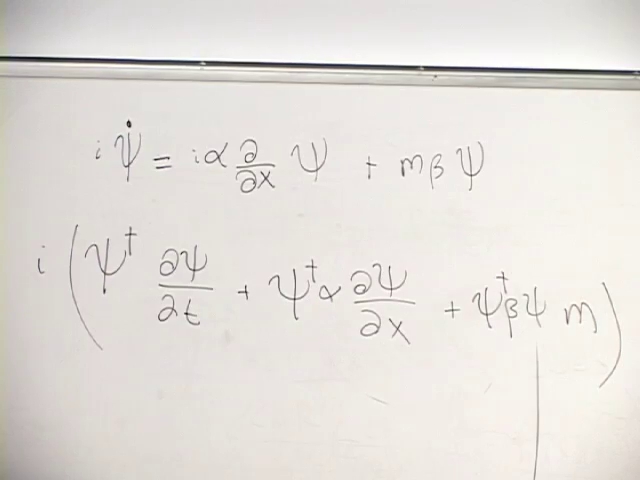
\includegraphics[width=0.76\textwidth]{lecture_09_figure_05.png}
\caption{Члены с временной производной, пространственной производной и массой в обсуждении поля Дирака.}
\lectureframe{00:25:37}
\end{figure}

\begin{classroomqa}
\lecturetimestamp{00:26:37}
\audiencequestion{Правильно ли поставлена скобка в пробном лагранжиане Дирака, так что \(i\) умножает все выражение?}
\lecturerresponse{Положение здесь уверенно не фиксируется, и для структурного пункта это не нужно: существует лагранжиан, порождающий уравнение Дирака.}
\end{classroomqa}

Теперь добавим скалярное поле \(\phi\). Наивное произведение \(\Psi^\dagger\Psi\,\phi\) не является лоренцевским скаляром. Если вставить ту же матрицу Дирака, которая входит в массовый член, получим
\begin{equation}
\mathcal L_{\mathrm{int}}
\propto
\Psi^\dagger\beta\Psi\,\phi.
\end{equation}
Эквивалентно, \(\Psi^\dagger\beta\Psi\) есть скалярная дираковская билинейная форма. Варьирование полного лагранжиана добавляет в уравнение Дирака член, пропорциональный \(\phi\), и в скалярное уравнение источник, пропорциональный \(\Psi^\dagger\beta\Psi\). Два поля рассеивают друг друга.

\begin{classroomqa}
\lecturetimestamp{00:28:03}
\audiencequestion{Является ли \(\beta\), вставляемая во взаимодействие скаляр--фермион, той же самой \(\beta\), что появляется в массовом члене Дирака?}
\lecturerresponse{Да. Это та же самая матрица Дирака.}
\end{classroomqa}

Сопоставление
\begin{equation}
m\Psi^\dagger\beta\Psi
\qquad\hbox{and}\qquad
\Psi^\dagger\beta\Psi\,\phi
\end{equation}
делает связь похожей на массовый параметр, замененный скалярным полем. К этому наблюдению мы вернемся, когда ближе к концу будет рассматриваться поле с ненулевым вакуумным значением.

До сих пор интерпретация была классической: волновые пакеты рассеивают другие волновые пакеты. Та же алгебра приобретает более четкий смысл в терминах частиц, когда поля становятся операторами.

\section{Что дают степени квантовых полей}

Реальное скалярное квантовое поле содержит и операторы рождения, и операторы уничтожения. Схематически,
\begin{equation}
\phi(x)\sim A^+(x)+A^-(x),
\end{equation}
где \(A^+\) создает квант, а \(A^-\) уничтожает квант. Следовательно, \(\phi^3(x)\) содержит четыре вида локального процесса:
\begin{equation}
\phi^3
\sim
(A^+)^3+(A^+)^2A^-+A^+(A^-)^2+(A^-)^3,
\end{equation}
где в этом схематическом прочтении детали упорядочения и численные коэффициенты опущены. Четыре изменения числа частиц таковы
\begin{equation}
3\longrightarrow0,
\qquad
0\longrightarrow3,
\qquad
2\longrightarrow1,
\qquad
1\longrightarrow2.
\end{equation}
Все три полевых множителя действуют в одной и той же точке \(x\). Поэтому один кубический член включает уничтожение 3 частиц, рождение 3 частиц, слияние 2 квантов в 1 и расщепление 1 кванта на 2. В физической амплитуде некоторые из этих локальных прочтений впоследствии могут быть устранены законом сохранения энергии--импульса, но все они присутствуют уже в самом операторном произведении.

У квадратичных свободных членов другая роль. Сначала опустим нормировку разности между соседними точками \(x\) и \(x'\):
\begin{equation}
\partial_x\phi
\ \propto\
\phi(x)-\phi(x').
\end{equation}
Возведение в квадрат и раскрытие скобок дает структуру членов
\begin{align}
\frac12(\partial_x\phi)^2
&\ \propto\
\frac12\bigl[\phi(x)-\phi(x')\bigr]^2
\\
&=
\frac12\phi(x)^2
+\frac12\phi(x')^2
-\phi(x)\phi(x').
\end{align}
Каждый квадрат в одной точке имеет несколько операторных прочтений: он может создать 2 кванта, уничтожить 2 или уничтожить один и снова создать его в той же точке. Эти члены не переносят частицу. Перекрестный член может уничтожить квант в \(x'\) и создать его в \(x\), или наоборот. Поэтому он действует как член перескока на ближайний соседний узел. Повторяющиеся множители переносят частицу из \(x\) в \(x'\), затем в \(x''\) и дальше. Квадратичные члены с производными управляют свободным распространением; кубические и более высокие члены рассеивают, создают и уничтожают частицы.

\begin{classroomqa}
\lecturetimestamp{00:36:07}
\audiencequestion{Должно ли конечно-разностное представление производной включать расстояние \(x-x'\)?}
\lecturerresponse{Да. Если обозначить это расстояние через \(L\), то после возведения разности в квадрат появляется множитель \(L^{-2}\). Этот численный множитель меняет коэффициент, но не интерпретацию как перескок.}
\end{classroomqa}

При восстановлении расстояния получаем
\begin{align}
\frac12(\partial_x\phi)^2
&\longrightarrow
\frac{1}{2L^2}\bigl[\phi(x)-\phi(x')\bigr]^2
\\
&=
\frac{1}{2L^2}\phi(x)^2
+\frac{1}{2L^2}\phi(x')^2
-\frac{1}{L^2}\phi(x)\phi(x').
\end{align}

Массовый член тоже квадратичен, но не содержит производной:
\begin{equation}
\frac12m^2\phi(x)^2.
\end{equation}
Его одночастичная интерпретация такова: входящий квант поглощается и вновь испускается в одной и той же точке. Он не перемещает квант; он придаёт вес, или в этом смысле учитывает, его присутствие там. Тот же квадрат оператора содержит также интерпретации с двумя рождениями и с двумя уничтожениями. Поэтому различие, существенное для движения, проходит между перекрёстным членом, соединяющим соседние точки, и массовой вставкой, действующей в пределах одной точки.

\section{Локальная вершина квантовой электродинамики}

Эти наброски элементарных процессов с частицами — зачатки диаграмм Фейнмана. Центральный пример — квантовая электродинамика, теория электронов, позитронов и фотонов.

Уравнение Дирака имеет моды с положительной и отрицательной энергией. В более старой терминологии \(\Psi\) содержит операторы уничтожения для обоих типов мод, а \(\Psi^\dagger\) содержит соответствующие операторы рождения. Удаление электрона с отрицательной энергией переинтерпретируется как рождение позитрона с положительной энергией. После этого переобозначения полезное схематическое разложение имеет вид
\begin{align}
\Psi
&\sim
C^-_{e^-}+C^+_{e^+},
\\
\Psi^\dagger
&\sim
C^+_{e^-}+C^-_{e^+}.
\end{align}
Тем самым \(\Psi\) уничтожает электрон или рождает позитрон, тогда как \(\Psi^\dagger\) рождает электрон или уничтожает позитрон. Это сокращение не подразумевает ни нормировки, ни спинового индекса, ни интеграла по импульсу.

Взаимодействие КЭД связывает дираковский ток с электромагнитным векторным потенциалом. В используемых здесь компонентных обозначениях его структура такова:
\begin{equation}
\mathcal L_{\mathrm{QED,int}}
\sim
e\left(
\Psi^\dagger\Psi\,A_0
+
\Psi^\dagger\boldsymbol{\alpha}\Psi\mathbin{\boldsymbol{\cdot}}\mathbf A
\right),
\end{equation}
где
\begin{equation}
J^0=\Psi^\dagger\Psi,
\qquad
\mathbf J=\Psi^\dagger\boldsymbol{\alpha}\Psi.
\end{equation}
Символ \(\sim\) важен: относительный знак между временным и пространственным членами зависит от соглашений о метрике и векторном потенциале. Инвариантное утверждение состоит в том, что четырёхток свёртывается с четырёхпотенциалом.\editorialnote{Источник фиксирует временную и пространственную компоненты тока, но не задаёт соглашение о метрике для свёртки компонент.}

Само фотонное поле \(A_\mu\) содержит операторы рождения и уничтожения фотонов. Его векторный характер также несёт поляризацию фотона---небольшой направленный ``флажок'' помимо его импульса.

\begin{classroomqa}
\lecturetimestamp{00:44:28}
\audiencequestion{Как взаимодействие может быть скаляром, если \(A_\mu\) — вектор, а фермионный множитель сначала кажется скаляром?}
\lecturerresponse{Фермионы тоже дают четырёхвектор: \(\Psi^\dagger\Psi\) — его временная компонента, а \(\Psi^\dagger\boldsymbol\alpha\Psi\) — пространственная. Свёртка этого тока с \(A_\mu\) даёт скаляр.}
\end{classroomqa}

Перемножение операторного содержания \(\Psi^\dagger\), \(\Psi\) и \(A_\mu\) даёт четыре привычные интерпретации одной локальной вершины:
\begin{enumerate}
\item электрон испускает фотон;
\item электрон поглощает фотон;
\item электрон и позитрон аннигилируют в фотон;
\item фотон рождает электрон--позитронную пару.
\end{enumerate}
Для первой интерпретации \(\Psi\) уничтожает входящий электрон, \(\Psi^\dagger\) рождает выходящий электрон, а фотонное поле рождает фотон. Если выбрать часть, уничтожающую фотон, получится поглощение. Если выбрать позитронные части, получится аннигиляция пары или рождение пары. В одном локальном члене содержится всё это семейство.

В диаграмме с фермионным потоком стрелка на линии позитрона направлена противоположно направлению распространения позитрона. При этом соглашении фермионная стрелка непрерывно проходит через каждую допустимую вершину КЭД. Четыре интерпретации различаются переносом внешних ножек между входящей и выходящей сторонами, а не разрывом линии фермионного потока.

Каждая из этих интерпретаций несёт один и тот же коэффициент \(e\), то есть электрический заряд в используемом микроскопическом соглашении. Этот коэффициент — электрический заряд \(e\), а не постоянная тонкой структуры, хотя эти величины тесно связаны. Амплитуда вершины пропорциональна \(e\); после учёта всех кинематических факторов и факторов нормировки соответствующий масштаб вероятности пропорционален \(e^2\).

\begin{classroomqa}
\lecturetimestamp{00:49:44}
\audiencequestion{Имеет ли интерпретация перехода фотона в электрон--позитрон тот же коэффициент, что и другие интерпретации вершины?}
\lecturerresponse{Да. Она несёт тот же коэффициент электрического заряда \(e\).}
\end{classroomqa}

\begin{classroomqa}
\lecturetimestamp{00:49:59}
\audiencequestion{Должен ли здесь быть масштабный множитель, раз вероятность не имеет размерности?}
\lecturerresponse{В используемом естественном микроскопическом соглашении заряд \(e\) безразмерен. Он задаёт масштаб амплитуды, а его квадрат задаёт масштаб вероятности.}
\end{classroomqa}

Конкретная картина такова: электрон ударяется о стенку и резко останавливается. Существует некоторая вероятность того, что энергия и импульс уйдут в виде фотона. Элементарный электромагнитный множитель в амплитуде такого излучения есть \(e\), поэтому масштаб его вероятности содержит \(e^2\). Это утверждение выделяет только фактор связи; реальная вероятность зависит также от состояния электрона и кинематики.

\begin{figure}[htbp]
\centering
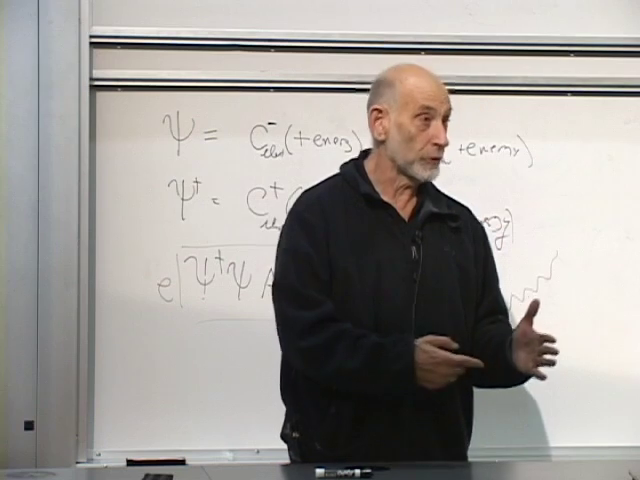
\includegraphics[width=0.78\textwidth]{lecture_09_figure_06.png}
\caption{Операторное содержание электронов и позитронов в \(\Psi\) и \(\Psi^\dagger\), с наброском электрон--фотонного взаимодействия.}
\lectureframe{00:50:39}
\end{figure}

\begin{classroomqa}
\lecturetimestamp{00:51:15}
\audiencequestion{Имеет ли электрический заряд единицы измерения?}
\lecturerresponse{Не в используемом здесь естественном микроскопическом соглашении. Макроскопический заряд часто выражают в кулонах, но в теории частиц заряд измеряют относительно выбранной элементарной единицы. В планковских или других естественных единицах эти величины выражаются как чистые числа.}
\end{classroomqa}

Различие здесь — в соглашениях и масштабах. Кулоны удобны для тока в проводах; безразмерная константа связи удобна для микроскопических амплитуд.\editorialnote{Краткий вопрос из 00:52:37--00:53:15 о ``группировке'' членов, несущих заряд, сильно повреждён и не допускает однозначной реконструкции.}

Все три поля в элементарном взаимодействии КЭД берутся в одной точке пространства-времени. Самой вершине не приписывается никакой внутренней временной задержки.

\begin{classroomqa}
\lecturetimestamp{00:53:19}
\audiencequestion{Являются ли поглощение и повторное испускание электрона, а также испускание фотона одновременными, или уравнение закладывает задержку?}
\lecturerresponse{В элементарной вершине все операторы берутся в одной и той же точке пространства-времени. Поэтому базовый процесс не содержит задержки между этими актами.}
\end{classroomqa}

\begin{classroomqa}
\lecturetimestamp{00:53:57}
\audiencequestion{Должна ли каждая из сохраняющихся величин сохраняться по отдельности?}
\lecturerresponse{Да. Электрический заряд — одна из величин, которые должны сохраняться по отдельности.}
\end{classroomqa}

Сохранение заряда видно и на диаграмме, и в алгебре. Процесс, который превращал бы входящий электрон в выходящий позитрон, менял бы знак заряда и не является допустимой вершиной КЭД. Если время направлено вверх, то стрелка электрона идёт вверх по времени, а стрелка позитрона направлена вниз; в допустимой вершине всегда есть сквозная фермионная стрелка. Алгебраически взаимодействие содержит один \(\Psi\) и один \(\Psi^\dagger\). Первый повышает заряд на одну единицу, когда уничтожает электрон или рождает позитрон, а второй понижает его на одну единицу. Их эффекты взаимно компенсируются.

\begin{classroomqa}
\lecturetimestamp{00:56:05}
\audiencequestion{Является ли заключённое в рамку электрон--фотонное выражение полным лагранжианом КЭД?}
\lecturerresponse{Нет. Это член взаимодействия. Квадратичные члены свободного фотона и квадратичные члены Дирака, которые управляют распространением, не выписаны.}
\end{classroomqa}

\begin{classroomqa}
\lecturetimestamp{00:56:35}
\audiencequestion{Выводится ли классический лагранжиан, тогда как квантовый лагранжиан угадывается и проверяется, и сохраняется ли в квантовой механике структура вида кинетическое минус потенциальное?}
\lecturerresponse{Схема кинетическое минус потенциальное сохраняется: временные производные задают кинетическую форму, пространственные градиенты её обобщают, а члены поля без производных задают потенциальную форму. Квантовый лагранжиан является более фундаментальным описанием. В состоянии, содержащем очень много квантов, тот же лагранжиан порождает классические волновые уравнения. Кандидатные лагранжианы предлагаются на основе физических принципов и более глубокой теории, а затем подтверждаются или отвергаются в экспериментах по столкновениям.}
\end{classroomqa}

Предел большой заселённости объясняет, почему одно и то же выражение может описывать квантовую теорию частиц и её классические волны. Это совпадение — не отдельное чудо, навязанное задним числом; классическое поле есть коллективное поведение многих квантов. И наоборот, экспериментальные столкновения достаточно непосредственно выявляют элементарные вершины, чтобы с большой точностью определять взаимодействия КЭД и Стандартной модели.

\section{Кроссинг и законы сохранения в пространстве-времени}

Внешние линии локальной вершины можно переносить между входящими и исходящими положениями. Исходящая частица, перенесенная на входящую сторону, переинтерпретируется как соответствующая ей античастица, и наоборот. В этом смысле один и тот же электрон--позитрон--фотонный оператор имеет прочтения, соответствующие испусканию, поглощению, аннигиляции пары, рождению пары и даже локальному прочтению со всеми входящими линиями.

\begin{classroomqa}
\lecturetimestamp{00:59:34}
\audiencequestion{Если диаграмму базовой вершины повернуть, останется ли она допустимым локальным прочтением?}
\lecturerresponse{Да. Ее внешние линии можно переносить между входящими и исходящими положениями с соответствующей переинтерпретацией частицы--античастицы.}
\end{classroomqa}

Локальное прочтение оператора еще не является полным физическим процессом. Его амплитуду нужно проинтегрировать по всем точкам пространства-времени, в которых могла бы возникнуть вершина. Интеграл по времени обеспечивает сохранение энергии, а интеграл по пространству — сохранение импульса. Картина, в которой электрон, позитрон и фотон все исчезают в вакуум, присутствует как формальное локальное прочтение, но проинтегрированная амплитуда обращается в нуль, потому что процесс не может сохранять энергию и импульс.

\begin{classroomqa}
\lecturetimestamp{01:00:30}
\audiencequestion{Означает ли картина со всеми входящими линиями, что электрон, позитрон и фотон могут исчезнуть в ничто?}
\lecturerresponse{Это прочтение локального оператора, но физическая амплитуда включает интегрирование по положению вершины. Эти интегралы налагают сохранение энергии и импульса, так что у этого кинематически запрещенного процесса амплитуда равна нулю.}
\end{classroomqa}

\begin{classroomqa}
\lecturetimestamp{01:01:57}
\audiencequestion{Существует ли и обратное прочтение из вакуума в электрон--позитрон--фотон, и исчезают ли запрещенные процессы после интегрирования?}
\lecturerresponse{Обратное локальное прочтение тоже присутствует. Интегрирование по пространству и времени устраняет любой процесс, несовместимый с законами сохранения.}
\end{classroomqa}

Производные в лагранжиане согласуются с операторным разложением без дифференцирования самих операторов рождения и уничтожения. Поле имеет схематический вид
\begin{equation}
\Psi(x)
\sim
\int d^3k\,
\bigl[
C(\mathbf k)e^{i\mathbf k\cdot\mathbf x-i\omega t}
+\cdots
\bigr].
\end{equation}
Операторы \(C(\mathbf k)\) служат коэффициентами в этом пространственно-временном разложении. Производные действуют на плоские волны, давая множители \(\mathbf k\) или \(\omega\).

\begin{classroomqa}
\lecturetimestamp{01:02:27}
\audiencequestion{При дифференцировании разложения поля дифференцируется ли сам оператор рождения?}
\lecturerresponse{Нет. В этом разложении операторы рождения и уничтожения не зависят от пространственно-временной координаты. Производные действуют на экспоненциальные множители и дают множители импульса и частоты.}
\end{classroomqa}

\section{Нуклоны и пионы как эффективная теория}

Тот же язык можно использовать для описания протонов, нейтронов и пионов. Протоны и нейтроны — фермионы, представляемые полями \(\Psi_p\) и \(\Psi_n\). Для этого обсуждения, посвященного подсчету взаимодействий, пионные поля рассматриваются как скалярные поля трех зарядовых разновидностей,
\begin{equation}
\pi^+,
\qquad
\pi^-,
\qquad
\pi^0.
\end{equation}
Протон и \(\pi^+\) несут одну положительную единицу электрического заряда, \(\pi^-\) несет одну отрицательную единицу, а нейтрон и \(\pi^0\) нейтральны. На более глубоком уровне пионы представляют собой кварк--антикварковые системы, но это внутреннее описание на первых порах можно оставить неуточненным.

Схематический список произведений нуклон--пионных полей, сохраняющих заряд, имеет вид
\begin{equation}
\mathcal L_{N\pi}
\sim
\left\{
\Psi_p^\dagger\Psi_n\,\pi^+,\;
\Psi_n^\dagger\Psi_p\,\pi^-,\;
\Psi_p^\dagger\Psi_p\,\pi^0,\;
\Psi_n^\dagger\Psi_n\,\pi^0
\right\}.
\end{equation}
Здесь показаны только состав полей и распределение зарядов; относительные коэффициенты, знаки и спинорно-матричная структура здесь не фиксируются. Заряд первого пионного поля фиксируется проверкой конкретного прочтения: нейтрон вместе с положительным пионом может дать протон, тогда как использование здесь отрицательного пиона привело бы к превращению отрицательного входящего заряда в положительный исходящий. Сопряженный член дает противоположно заряженный процесс.\editorialnote{Знак пиона в источнике исправляется несколько раз, прежде чем получается сохраняющая заряд пара, показанная здесь; приведенный порядок фиксирует эту окончательную схематическую структуру.}

Каждый член снова имеет несколько скрещенных прочтений. Перенос исходящего нейтрона на входящую сторону превращает его во входящий антинейтрон. Поэтому заряженная вершина может описывать протон и антинейтрон, образующие \(\pi^+\), а также процессы типа \(p\to n+\pi^+\), когда это допускает кинематика. Нейтральные члены позволяют протону или нейтрону испускать или поглощать \(\pi^0\). Сохранение заряда отбирает допустимое семейство, тогда как энергия, импульс и любые дополнительные симметрии определяют, какой его представитель может происходить в конкретном эксперименте.

Это было полезным эффективным описанием до того, как стала известна кварковая субструктура. Оно остается полезным всякий раз, когда зонд не может разрешить эту структуру. Протон обладает конечным пространственным распределением своих составляющих, подобно тому как атом имеет внутреннюю структуру, хотя и в гораздо меньшем масштабе. Если в эксперименте перенос импульса слишком мал, чтобы разрушить протон или разрешить его структуру, протон можно рассматривать как точечную частицу со своим собственным полем. Достаточно жесткое столкновение выявляет кварки, и тогда поле протона как точечной частицы уже неадекватно.

Поскольку протон несет заряд, у него также есть локальное протон--фотонное взаимодействие, схематически \(J_p^\mu A_\mu\), где \(J_p^\mu\) — протонный ток. У электрона есть соответствующее ему электрон--фотонное взаимодействие. Однако протон не может превратиться в нейтрон, испустив фотон: \(p\to n+\gamma\) нарушает сохранение заряда.

\begin{classroomqa}
\lecturetimestamp{01:10:28}
\audiencequestion{Что происходит, когда взаимодействуют протон и электрон?}
\lecturerresponse{У каждой заряженной частицы есть фотонная вершина. Протон может испустить фотон, оставаясь протоном, а электрон может поглотить фотон, оставаясь электроном. Протон--электронное рассеяние строится из этих двух локальных вершин и распространения фотона между ними.}
\end{classroomqa}

\section{Локальность и повторение элементарных процессов}

Для полного протон--электронного обмена нет специального нелокального члена. Одна локальная вершина испускает фотон в точке протона, квадратичные фотонные члены переносят его от соседней точки к соседней, а другая локальная вершина поглощает его в точке электрона. Протяженный процесс является произведением этих элементарных звеньев.
\begin{equation}
\begin{aligned}
\bigl[J_p^\mu A_\mu\bigr](x_p)
&\longrightarrow
\underbrace{x_p\to x_1\to x_2\to\cdots\to x_e}_{\text{quadratic photon propagation}}
\\
&\longrightarrow
\bigl[J_e^\nu A_\nu\bigr](x_e).
\end{aligned}
\end{equation}
Стрелки в этой схематической цепочке обозначают последовательные вставки в соседних точках, а не новое нелокальное взаимодействие.

\begin{classroomqa}
\lecturetimestamp{01:12:06}
\audiencequestion{Как записать лагранжиан для всего протон--электронного обмена?}
\lecturerresponse{Не добавляют отдельный член для всего протяженного события. Оно строится из локальной протон--фотонной вершины, повторяющихся квадратичных членов распространения и локальной электрон--фотонной вершины.}
\end{classroomqa}

Локальная структура имеет две формы. Член взаимодействия без производных действует в одной точке пространства-времени. Член с производной, записанный в виде конечной разности, связывает эту точку только с соседней точкой. Ни один из этих типов не переносит частицу непосредственно на конечное расстояние. Распространение на большие расстояния складывается из многих бесконечно малых шагов; элементарного действия на расстоянии нет.

\begin{classroomqa}
\lecturetimestamp{01:14:36}
\audiencequestion{Содержит ли лагранжиан члены только в одной точке?}
\lecturerresponse{Члены взаимодействия действуют в одной точке. Члены с производными связывают одну точку с бесконечно близкой соседней точкой. Испускание, множество переходов между соседними точками и поглощение вместе создают обмен на конечное расстояние.}
\end{classroomqa}

\begin{classroomqa}
\lecturetimestamp{01:15:36}
\audiencequestion{Присутствуют ли все составляющие протяженного процесса, и означает ли их составление умножение?}
\lecturerresponse{Да. Каждое элементарное испускание, переход или поглощение закодировано в лагранжиане. Произведения повторных вставок объединяют эти части в более крупный процесс.}
\end{classroomqa}

Обсуждаемая релятивистская квантовая теория поля предполагает заданный пространственно-временной фон, на котором определены ее поля. Ее не следует смешивать с полной квантовой теорией динамической геометрии пространства-времени.

\begin{classroomqa}
\lecturetimestamp{01:16:28}
\audiencequestion{Остается ли такое составление справедливым в сильно релятивистской обстановке, например вблизи горизонта черной дыры?}
\lecturerresponse{Расширение на случай черной дыры выходит за рамки этой конструкции. Используемая здесь квантовая теория поля сама по себе не дает полного описания динамики черной дыры, где существенна гравитация.}
\end{classroomqa}

Поле — это оператор элементарного локального акта. Один множитель поля может поглотить частицу или испустить ее. Произведение двух множителей может поглотить одну частицу и испустить другую в той же точке; более высокие произведения могут еще сильнее изменить состав частиц. Произведения локальных операторов соединяют эти акты в истории. В пространстве-времени движение представляется как поглощение в одной малой области, переиспускание в соседнюю область, еще одно поглощение и еще одно переиспускание. Предел, в котором размер шага стремится к нулю, а число шагов растет, дает непрерывную траекторию.

\begin{classroomqa}
\lecturetimestamp{01:17:30}
\audiencequestion{Как следует понимать поля, расстояние и время в этой картине локальных шагов?}
\lecturerresponse{Поля — это операторы локального поглощения и испускания. Произведения связывают эти элементарные акты, а движение в пространстве-времени строится из бесконечно малых шагов между соседними точками до перехода к пределу континуума.}
\end{classroomqa}

Регуляризованной отправной точкой поэтому служит разбиение пространства-времени на малые ячейки, к которым привязаны полевые операторы.\editorialnote{Формулировка вопроса из аудитории на 01:17:30--01:20:40 частично неразборчива; перефразированный вопрос сохраняет лишь ту тему, которую удаётся восстановить, тогда как ответ о локальных операторах и последовательных шагах в пространстве-времени ясен.} Производные превращаются в разности. Квадратичные перекрёстные члены связывают соседние ячейки, тогда как массовые члены и члены взаимодействия действуют внутри одной ячейки. Ячейки служат средством задания предельной теории, а не дополнительными частицами и не новой физической шкалой масс.

Эффекты специальной теории относительности не нужно добавлять отдельно на каждом шаге. Если лагранжиан является скаляром Лоренца, то построенные из него амплитуды лоренц-инвариантны, и такие эффекты, как замедление времени, следуют из этой структуры.

\begin{classroomqa}
\lecturetimestamp{01:21:10}
\audiencequestion{Создают ли движение с высокой энергией и замедление времени дополнительные проблемы в многошаговом процессе?}
\lecturerresponse{Отдельная поправка не требуется. Если лагранжиан является скаляром Лоренца, то специальные релятивистские эффекты, такие как замедление времени, уже встроены в результат. В остальном точный смысл опасения, стоящего за этим вопросом, не вполне ясен.}
\end{classroomqa}

Операторы рождения и уничтожения могут быть представлены в координатном базисе или в базисе импульсов. Оператор рождения в координатном пространстве представляет собой суперпозицию Фурье операторов рождения в импульсном пространстве, и наоборот. Не существует оператора, который создавал бы состояние с одновременно точно заданными координатой и импульсом. Чтобы резко локализовать частицу, требуется широкий диапазон импульсов; резкая локализация по импульсу размазывает её по координате. Связь Фурье между этими двумя базисами и есть принцип неопределённости на этом языке.

\begin{classroomqa}
\lecturetimestamp{01:22:48}
\audiencequestion{Как операторы рождения и уничтожения связаны с координатой, импульсом и принципом неопределённости?}
\lecturerresponse{Они могут быть представлены как функции координаты или как функции импульса. Эти два представления связаны преобразованием Фурье. Резко локализованное по координате состояние требует многих импульсов, тогда как состояние, резко локализованное по импульсу, размазано по координате; оператора рождения для одновременно точно заданных \(x\) и \(p\) не существует.}
\end{classroomqa}

Построение на ячейках теперь можно сформулировать полностью. Обозначьте ячейки индексом \(n\), замените производную конечной разностью, например
\begin{equation}
\partial_\mu\phi(x)
\longrightarrow
\frac{\phi_{n+\hat\mu}-\phi_n}{a},
\end{equation}
и поместите в каждую ячейку все виды полей. Квадратичный перекрёстный член уничтожает квант в одной ячейке и создаёт его в соседней. Теория континуума получается при устремлении шага \(a\) к нулю после того, как регуляризованные выражения определены.
\begin{equation}
\underbrace{\phi_n\phi_{n+\hat\mu}}_{\text{hop }n\leftrightarrow n+\hat\mu},
\qquad
\underbrace{m^2\phi_n^2}_{\text{same-cell mass insertion}}.
\end{equation}

\begin{classroomqa}
\lecturetimestamp{01:25:16}
\audiencequestion{Можно ли теперь полностью сформулировать разбиение пространства-времени на ячейки?}
\lecturerresponse{Да. Поля индексируются ячейками, производные заменяются конечными разностями, а квадратичные члены переводят частицы между соседними ячейками. Континуум восстанавливается, когда размер ячейки стремится к нулю.}
\end{classroomqa}

Электроны переходят между ячейками благодаря своим квадратичным членам, и фотоны — тоже. Когда электрон и фотон встречаются в одной ячейке, взаимодействие КЭД может поглотить и вновь испустить электрон, одновременно создавая или уничтожая фотон. Скалярный массовый член допускает внутриклеточную интерпретацию: частица входит в эту ячейку и выходит из неё с коэффициентом, пропорциональным \(m^2\). Этот член не обеспечивает перехода между ячейками.

\begin{classroomqa}
\lecturetimestamp{01:28:18}
\audiencequestion{Связан ли размер ячейки с массовым коэффициентом?}
\lecturerresponse{Нет. Размер ячейки — это шаг регуляризации, который в конечном счёте устремляется к нулю; массовый коэффициент является независимым параметром лагранжиана.}
\end{classroomqa}

\begin{classroomqa}
\lecturetimestamp{01:28:43}
\audiencequestion{Является ли перемножение локальных множителей построением совместной амплитуды по пространству-времени, а не просто последовательностью во времени?}
\lecturerresponse{Да. Ячейки покрывают пространство-время, и их локальные вклады объединяются по всей этой пространственно-временной решётке. Произведение даёт совместную амплитуду для требуемых локальных событий и шагов распространения.}
\end{classroomqa}

\section{Источники, детекторы и динамика между ними}

Полный процесс — это история в пространстве-времени. Его начальное условие задаётся тем, что подготавливает экспериментатор, а конечное — тем, что регистрируют детекторы. Простым источником служит нагретая нить, испускающая электрон. Полевой оператор на нити создаёт этот входящий электрон; полевые операторы в положениях детекторов описывают его последующее поглощение.

\begin{classroomqa}
\lecturetimestamp{01:29:30}
\audiencequestion{Какова начальная стадия такого пространственно-временного процесса?}
\lecturerresponse{Она подготавливается у источников. Простой пример — электрон, испускаемый нагретой нитью: полевой оператор на нити создаёт электрон, а полевые операторы у детекторов задают конечные события поглощения.}
\end{classroomqa}

То же построение можно сформулировать, начиная с вакуума. Операторы рождения у источников строят входящее состояние над вакуумом. Операторы уничтожения, связанные с детекторами, выделяют исходящее состояние. Эти операторы задают граничные условия; они не заменяют динамику во всей области между источником и детектором.

\begin{classroomqa}
\lecturetimestamp{01:31:11}
\audiencequestion{Было бы неверно помещать динамику только в источники, испускающие частицы, а не во всю систему?}
\lecturerresponse{Да. Начните с вакуума, используйте операторы источников, чтобы подготовить входящие частицы, и операторы детекторов, чтобы выделить конечные частицы. Между ними повторные вставки лагранжиана действуют по всему пространству-времени, перемещая частицы, создавая их и уничтожая.}
\end{classroomqa}

При достаточном числе вставок несколько частиц могут одновременно проходить через много соседних ячеек; по пути частицы также могут создаваться или уничтожаться. Начальные операторы задают, что входит, конечные — что регистрируется, а повторные вставки лагранжиана задают всё, что происходит между ними.

\begin{classroomqa}
\lecturetimestamp{01:33:24}
\audiencequestion{Если может происходить сколь угодно много вставок лагранжиана, интегрируется ли по их положениям?}
\lecturerresponse{Да. Интегрирование ведётся по их пространственно-временным положениям. Точные правила Фейнмана здесь не выводятся; непосредственная мысль состоит в том, что простые локальные полевые выражения кодируют примитивные взаимодействия, из которых собирается полный процесс.}
\end{classroomqa}

\section{Фазовая симметрия, заряд и амплитуды}

Запись примитивных процессов в лагранжиане также делает видимыми их симметрии. Рассмотрим глобальное фазовое преобразование электронного поля,
\begin{equation}
\Psi\longrightarrow e^{i\theta}\Psi,
\qquad
\Psi^\dagger\longrightarrow e^{-i\theta}\Psi^\dagger,
\qquad
A_\mu\longrightarrow A_\mu.
\end{equation}
Член с равным числом \(\Psi\) и \(\Psi^\dagger\) не меняется, поскольку фазы сокращаются. Член с неравным их числом приобрёл бы фазовый множитель. Равенство этих чисел — алгебраическая форма закона сохранения заряда.

Это одно из центральных преимуществ лагранжева описания. Его полевые множители показывают элементарные процессы, их комбинации — симметрии, а симметрии — законы сохранения. Повторные вставки переводят подготовленное начальное состояние в выбранное конечное состояние. Результатом является квантовая амплитуда. Для точного вычисления нужны правила Фейнмана, но структурное содержание уже видно: локальные операции повторяются во всех порядках, разрешённых законами сохранения.

\section{Измерения полей и коммутаторы}

Полевые операторы сохраняют обычный квантово-механический смысл операторов. Их собственные значения — возможные результаты измерений поля, а собственные векторы описывают состояния, соответствующие этим значениям. Электрическое поле можно исследовать, поместив в него заряженную частицу и наблюдая, как она ускоряется.

\begin{classroomqa}
\lecturetimestamp{01:37:06}
\audiencequestion{Играют ли собственные значения и собственные векторы полевых операторов свою обычную квантово-механическую роль?}
\lecturerresponse{Да. Собственные значения — это возможные измеренные значения поля, а поля можно исследовать по их воздействию на частицы. Коммутаторы определяют ограничения на одновременные измерения.}
\end{classroomqa}

Тривиальное тождество
\begin{equation}
[\phi(x),\phi(x)]=0
\end{equation}
не решает вопроса об измерении. Нужно указать две наблюдаемые величины и их пространственно-временное отношение. Поле и его сопряжённый импульс образуют каноническую некоммутирующую пару, и операторы поля в точках, разделённых времениподобным интервалом, не обязаны коммутировать; локальные бозонные поля при пространственноподобном разделении коммутируют, как и требует локальность. Поэтому привычная связь между коммутаторами и неопределённостью сохраняется, но только после того, как пара операторов правильно определена.\editorialnote{В источнике утверждение о некоммутативности в различных точках сформулировано слишком широко. Это уточнение сохраняет его мысль об измерении, одновременно обеспечивая микропричинность локальных бозонных полей при пространственноподобном разделении.}

\begin{classroomqa}
\lecturetimestamp{01:39:57}
\audiencequestion{Электрическое, или электромагнитное, поле измеряется в вольтах или в вольтах на метр?}
\lecturerresponse{Электрическое поле измеряется в вольтах на метр. Вольты и метры — не самый полезный язык для микроскопических полевых процессов, которые естественнее описывать через фотоны. И наоборот, квантовая теория поля — не самый полезный язык для решения вопроса, как поливать дом.}
\end{classroomqa}

Единицы, естественные для одного описания, не обязательно окажутся наиболее наглядными в другом. Вольты и вольты на метр подходят для макроскопической аппаратуры; описание через рождение и уничтожение фотонов подходит для микроскопических процессов.

\begin{classroomqa}
\lecturetimestamp{01:41:10}
\audiencequestion{Центральная идея состоит в том, что члены лагранжиана — это строительные блоки, объединяемые в более крупные процессы?}
\lecturerresponse{Да. Элементарные процессы повторяются от точки к точке. Каждый базовый элемент действует в одной точке пространства-времени или связывает соседние точки через член с производной. Кажущееся нелокальным распространение строится из этих локальных шагов; элементарного дальнодействия нет.}
\end{classroomqa}

\section{Произведения локальных процессов и суммы по путям}

Существует компактный эвристический способ показать повторение локальных процессов. Разобьём пространство-время на ячейки и запишем
\begin{equation}
\prod_x\bigl(1+\mathcal L_I(x)\bigr),
\end{equation}
где \(x\) обозначает ячейки, а \(\mathcal L_I(x)\) — локальный лагранжиан взаимодействия. Это не точная формула непрерывного случая. Это комбинаторная схема-заменитель, показывающая, как произведения порождают любой допустимый набор локальных событий.

\begin{classroomqa}
\lecturetimestamp{01:42:18}
\audiencequestion{Можно ли много шагов рождения, распространения и уничтожения свести к одному выражению?}
\lecturerresponse{Эвристически нужно взять по одному множителю \(1+\mathcal L_I(x)\) для каждой ячейки пространства-времени. При разложении произведения получаются либо отсутствие события, либо одно событие в любой выбранной точке, либо события в нескольких точках.}
\end{classroomqa}

Для двух ячеек,
\begin{align}
\bigl(1+\mathcal L_I(x)\bigr)
\bigl(1+\mathcal L_I(x')\bigr)
&=
1+\mathcal L_I(x)+\mathcal L_I(x')
\notag\\
&\quad{}+\mathcal L_I(x)\mathcal L_I(x').
\end{align}
Первый член означает, что ни одно из взаимодействий не происходит. Следующие два помещают одно элементарное взаимодействие в \(x\) или в \(x'\). Последний член помещает взаимодействия в обе точки. При большом числе множителей возникают члены с одной точкой, двумя точками, тремя точками и так далее. Член с несколькими вершинами может описывать, например, процесс, в котором две входящие частицы порождают три выходящие частицы.

Квадратичные члены, отвечающие за распространение, входят в ту же конструкцию. Конечное смещение представляется цепочкой соседних вставок. Где-то в разложенном произведении присутствуют множители в одной ячейке, в соседней с ней, в следующей соседней и так далее, переносящие частицу между начальной и конечной точками.

\begin{classroomqa}
\lecturetimestamp{01:46:29}
\audiencequestion{Если для конечного распространения требуется много локальных членов, описывающих движение, то как восстанавливается нужное перемещение?}
\lecturerresponse{Большое произведение содержит цепочки соседних вставок, которые переносят частицу из её начальной точки в конечную. Обычно существует много таких цепочек вдоль разных путей. Каждый путь вносит вклад в амплитуду, а полная амплитуда есть их сумма.}
\end{classroomqa}

Если \(r\) обозначает путь, то схематически
\begin{equation}
\mathcal A_{\mathrm{total}}=\sum_r\mathcal A_r,
\qquad
P=\left|\mathcal A_{\mathrm{total}}\right|^2.
\end{equation}
Обычные вероятности не приписываются путям с последующим суммированием. Сначала складываются амплитуды:
\begin{equation}
\left|\sum_r\mathcal A_r\right|^2
=
\sum_r|\mathcal A_r|^2
+
\sum_{r\ne s}\mathcal A_r\mathcal A_s^*.
\end{equation}
Перекрёстные члены и есть интерференция.

\begin{classroomqa}
\lecturetimestamp{01:48:27}
\audiencequestion{Согласуется ли это с опытом с двумя щелями?}
\lecturerresponse{Именно. Альтернативы прохождения через две щели вносят амплитуды. Квадрат их суммы порождает интерференционные члены — точно так же, как интерферируют многие пространственно-временные пути в конструкции с локальными шагами.}
\end{classroomqa}

\begin{classroomqa}
\lecturetimestamp{01:49:00}
\audiencequestion{Откуда берётся \(1\) в каждом множителе \(1+\mathcal L_I\)?}
\lecturerresponse{Это комбинаторный приём, позволяющий ячейке вносить вклад как без взаимодействия, так и с взаимодействием. Он связан с методами интеграла по траекториям, но выписанное произведение — лишь эвристическое приближение к техническому выражению.}
\end{classroomqa}

Точный формализм обеспечивает корректные интегрирования по пространству-времени, упорядочение, нормировку и фазы. Произведение полезно потому, что выявляет комбинации, не выдавая себя за полный формализм.

\begin{classroomqa}
\lecturetimestamp{01:49:57}
\audiencequestion{Это принцип стационарного действия?}
\lecturerresponse{Нет. В классической механике стационарность действия выделяет особую классическую траекторию. Квантовая механика вместо этого суммирует амплитуды по траекториям, причём их веса определяются действием. Даже чрезвычайно окольный путь---через Париж по дороге из офиса в соседний дом---входит в квантовую сумму.}
\end{classroomqa}

Контраст прост, хотя связь здесь тонка. Классическая механика выбирает стационарную траекторию. Квантовая механика суммирует по траекториям; в подходящем пределе фазы усиливают друг друга вблизи классической траектории.

\section{Восстановление лагранжиана и выбор сектора}

Как только заданы лагранжиан и конкретный процесс, правила вычисления его вероятности однозначны. Само вычисление всё ещё может требовать изобретательности, как это часто бывает в трудной математике, но более глубокая неопределённость заключается в выяснении того, какие поля и константы связи использует природа.

\begin{classroomqa}
\lecturetimestamp{01:50:43}
\audiencequestion{Искусство — в том, чтобы записать лагранжиан, или в том, чтобы им пользоваться?}
\lecturerresponse{Главное искусство состоит в восстановлении лагранжиана по экспериментальным данным. Как только он известен, для процесса, в котором, например, две частицы входят, а четыре выходят, существует определённая амплитуда, вычисляемая по точным правилам. Выполнение самих математических выкладок может потребовать изобретательности, но это не неоднозначность теории.}
\end{classroomqa}

Столкновения частиц выявляют элементарные вершины. Предлагаются члены, часто подсказываемые симметрией и более глубокими принципами, а получающиеся амплитуды сопоставляются с наблюдаемыми результатами. Успех фиксирует и допустимые комбинации полей, и их численные коэффициенты.

\begin{classroomqa}
\lecturetimestamp{01:52:24}
\audiencequestion{Есть ли отдельный лагранжиан для каждого взаимодействия---большая книга лагранжианов?}
\lecturerresponse{Рабочая картина иная: один большой лагранжиан, содержащий все поля и взаимодействия, хотя эта картина в конечном счёте может оказаться ложной. Различимые сектора проявляются как части суммы. Новая частица добавляет поле; новый элементарный процесс добавляет член взаимодействия.}
\end{classroomqa}

Полное выражение может быть громоздким, не занимая при этом целую книгу. В качестве намеренно грубой оценки можно представить себе порядка сотни объектов, называемых элементарными частицами, и несколько сотен членов. Квантовая электродинамика, сильное и слабое взаимодействия и гравитационный сектор всё же могли бы уместиться всего на нескольких плотно исписанных страницах. Точное число здесь несущественно. Рабочая картина состоит в одном динамическом выражении, собранном из многих различимых частей, и подчёркнуто, что это лишь картина, которая со временем может оказаться неполной.

Вопрос о том, определяют ли поля более фундаментальную геометрию пространства-времени, выходит за рамки стандартной квантово-полевой схемы, используемой здесь.\editorialnote{Вопрос в 01:55:00--01:55:20 слишком повреждён, чтобы можно было надёжно определить многообразие или геометрическую конструкцию; надёжным остаётся только этот ответ о границах рассматриваемой темы.}

\begin{classroomqa}
\lecturetimestamp{01:55:22}
\audiencequestion{Числа, определяемые экспериментально, — это константы связи?}
\lecturerresponse{Константы связи — это коэффициенты при членах лагранжиана. Коэффициент \(m^2\) при квадратичном массовом члене — один пример; коэффициенты при \(\phi^4\), \(\phi^6\) или ещё более высоких степенях — другие.}
\end{classroomqa}

Один коэффициент контролирует целое семейство связанных амплитуд, потому что каждое произведение полей допускает несколько прочтений в терминах рождения и уничтожения. Поэтому знание лагранжиана определяет гораздо больше, чем одну изолированную реакцию.

\begin{classroomqa}
\lecturetimestamp{01:56:05}
\audiencequestion{Нужно ли знать весь лагранжиан, чтобы рассчитывать квантовую электродинамику?}
\lecturerresponse{Бесконечная точность потребовала бы учёта каждого сектора, через который могут взаимодействовать электроны и фотоны. Однако при атомных энергиях электрон--фотонный сектор обычно можно выделить. Энергии недостаточно, чтобы разрешить тонкую кварковую структуру, поэтому другими секторами можно пренебречь с требуемой точностью.}
\end{classroomqa}

Практические вычисления используют сектор, соответствующий экспериментальному масштабу. Это похоже на гидродинамику: сложная микроскопическая система может допускать точное крупнозернистое описание без явного представления всех своих более глубоких составляющих. Поэтому квантовая теория поля может быть одновременно---феноменологической в полях и коэффициентах, определяемых из эксперимента, и точной в правилах, применяемых после задания этих ингредиентов.

\begin{classroomqa}
\lecturetimestamp{01:58:09}
\audiencequestion{Включает ли Стандартная модель гравитацию, и включают ли эти релятивистские лагранжианы общую теорию относительности?}
\lecturerresponse{Теория, официально называемая Стандартной моделью, не включает гравитацию, хотя при обсуждении более широкой теории гравитацию можно добавить. Рассматриваемые здесь теории поля объединяют квантовую механику со специальной теорией относительности. Сами по себе они не включают общую теорию относительности.}
\end{classroomqa}

\section{Вакуумное значение как коэффициент массы}

Масса скалярного поля выступает как коэффициент при \(\phi^2\). Поэтому взаимодействие с другим полем может имитировать массовый член, когда это другое поле имеет ненулевое вакуумное значение.

\begin{classroomqa}
\lecturetimestamp{01:59:16}
\audiencequestion{Если массы частиц возникают благодаря взаимодействиям Хиггса, может ли хиггсовское взаимодействие играть роль массового члена?}
\lecturerresponse{Да. Член \(H\phi^2\) кубичен и обычно представляет взаимодействие с двумя линиями \(\phi\) и одной линией \(H\). Если потенциал \(V(H)\) выбирает вакуум с ненулевым значением поля \(H\), это вакуумное значение является числом, умножающим \(\phi^2\), так что оно даёт эффективный квадратичный массовый член.}
\end{classroomqa}

Рассмотрим схематически
\begin{equation}
\mathcal L\supset H\phi^2-V(H).
\end{equation}
Как операторный член, \(H\phi^2\) может поглотить квант \(\phi\), испустить квант \(\phi\), а также испустить или поглотить квант \(H\). Предположим, что потенциал имеет два минимума вдали от \(H=0\), и вакуум выбирает один из них:
\begin{equation}
\langle H\rangle=v\ne0.
\end{equation}
Запишем поле как сумму его вакуумного значения и флуктуации,
\begin{equation}
H=v+h.
\end{equation}
Тогда
\begin{equation}
H\phi^2=v\phi^2+h\phi^2.
\end{equation}
Первый член квадратичен по \(\phi\) и вносит вклад в коэффициент массы этого поля; второй остаётся взаимодействием с флуктуирующим полем \(h\).\editorialnote{В источнике предложение заканчивается утверждением, что ненулевое вакуумное значение становится коэффициентом массы. Показанная подстановка является непосредственным алгебраическим завершением; её нормировка и знак зависят от соглашений для полного лагранжиана.}

\begin{classroomqa}
\lecturetimestamp{02:01:29}
\audiencequestion{Включает ли Стандартная модель рождение и уничтожение виртуальных частиц?}
\lecturerresponse{Безусловно. Виртуальное рождение и уничтожение внутренне присущи повторяющимся квантовым процессам, закодированным в лагранжиане Стандартной модели.}
\end{classroomqa}